\documentclass{beamer}

\definecolor{dgreen}{rgb}{0.,0.6,0.}

\usefonttheme{professionalfonts} % using non standard fonts for beamer
\usefonttheme{serif} % default family is serif
\usepackage{fontspec}
%\setmainfont{Liberation Serif}
%\setmainfont{Myriad Pro}

\setmainfont[
   ItalicFont     = HelveticaNeue-Italic,
   BoldFont       = HelveticaNeue-Bold,
   BoldItalicFont = HelveticaNeue-BoldItalic]{HelveticaNeue-Light}
\newfontfamily\NHLight[
   ItalicFont     = HelveticaNeue-LightItalic,
   BoldFont       = HelveticaNeue-UltraLight,
   BoldItalicFont = HelveticaNeue-UltraLightItalic]{HelveticaNeue-Light}
   
\setbeamertemplate{frametitle}[default][center]
\setbeamertemplate{itemize item}{\textemdash}

\setbeamercolor{frametitle}{fg=black}
\setbeamerfont{frametitle}{size=\LARGE,family=\NHLight,series=\bfseries\itshape}

\usepackage{algorithmic}
\usepackage{graphicx}
\usepackage{subfig}
\usepackage{natbib}
\usepackage{pifont}
 \usepackage{overpic}
% \usepackage{beamer}
% Schweinsberg: time varying KC
\newcommand{\todo}[1]{\textcolor{red}{[#1]}}


\newcommand\textrmlf[1]{{\NHLight#1}}
\newcommand\textitlf[1]{{\NHLight\itshape#1}}
\let\textbflf\textrm
\newcommand\textulf[1]{{\NHLight\bfseries#1}}
\newcommand\textuitlf[1]{{\NHLight\bfseries\itshape#1}}

\newcommand*{\TitleFont}{%
      \usefont{\encodingdefault}{\rmdefault}{b}{n}%
      \fontsize{30}{30}%
      \selectfont}
      
      

\graphicspath{{../figures/}}

\title{\TitleFont \textuitlf{Genetic regulation of doxorubicin response in cardiomyocytes}}
\author{David A. Knowles, John D. Blischak, Courtney Burrows}

\usepackage{tikz}
\usetikzlibrary{arrows,decorations.pathreplacing,shapes}
\tikzset{>=stealth'}
\tikzstyle{graphnode} = [circle,draw=black,minimum size=15pt,text width=10pt,text centered] 
\tikzstyle{var}   =[graphnode,fill=white]
\tikzstyle{obs}   =[graphnode,fill=lightgray]
\tikzstyle{fac}   =[rectangle,draw=black,fill=black!25,minimum size=5pt]
\tikzstyle{edge}  =[draw,-]
\tikzstyle{prior} =[rectangle, draw=black, fill=black, minimum size = 10pt]
\tikzstyle{dirprior} = [circle, draw=black, fill=black, minimum size=5pt]
\begin{document}

\begin{frame}
\titlepage
\end{frame}

\begin{frame}{Why?}
\begin{itemize}
\item Doxorubicin is an anthracycline, a class of chemotherapy drugs which intercalate DNA preventing replication
\item Used against a broad range of both solid and blood cancers, often in combination with other drugs
\item However, at high doses 36\% of patients develop cardiomyopathies leading to heart failure
\end{itemize}
\end{frame}

\begin{frame}{iPSC-derived cardiomyocytes}
\begin{itemize}
\item The Gilad lab transformed 76 Hutterite samples: 
$$ \text{Blood draw} \Rightarrow \text{LCL} \Rightarrow \text{iPSC} \Rightarrow \text{Cardiomyocyte} $$
\item iPSCs recover more donor specific expression \citep{Thomas2015} and have negligible precursor cell-type effects \citep{Burrows2016}
\item Appealing model system for querying the genetics of human disease
\end{itemize}
\end{frame}

\begin{frame}{Treatment with doxorubicin (pilot)}
\begin{itemize}
\item Four cell lines, $2x$ technical replicates. Microarrays. 
\end{itemize}
\centering
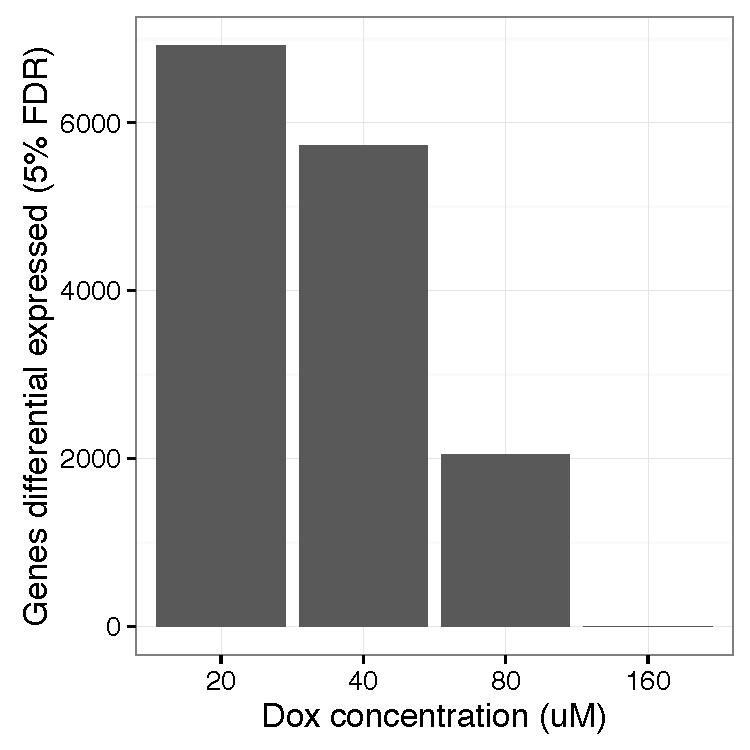
\includegraphics[width=.7\textwidth,clip,trim=0 0 0 0]{../figures/pilot_de.pdf}
\end{frame}

\begin{frame}{RNA-sequencing}
\begin{itemize}
\item 50bp single end on HiSeq 4000 [two rounds]
\item QC using fastqc and multi\_qc. 
\item Mapped to GRCh38 using STAR
\item Require 10M exonic reads per sample
\end{itemize}
\centering
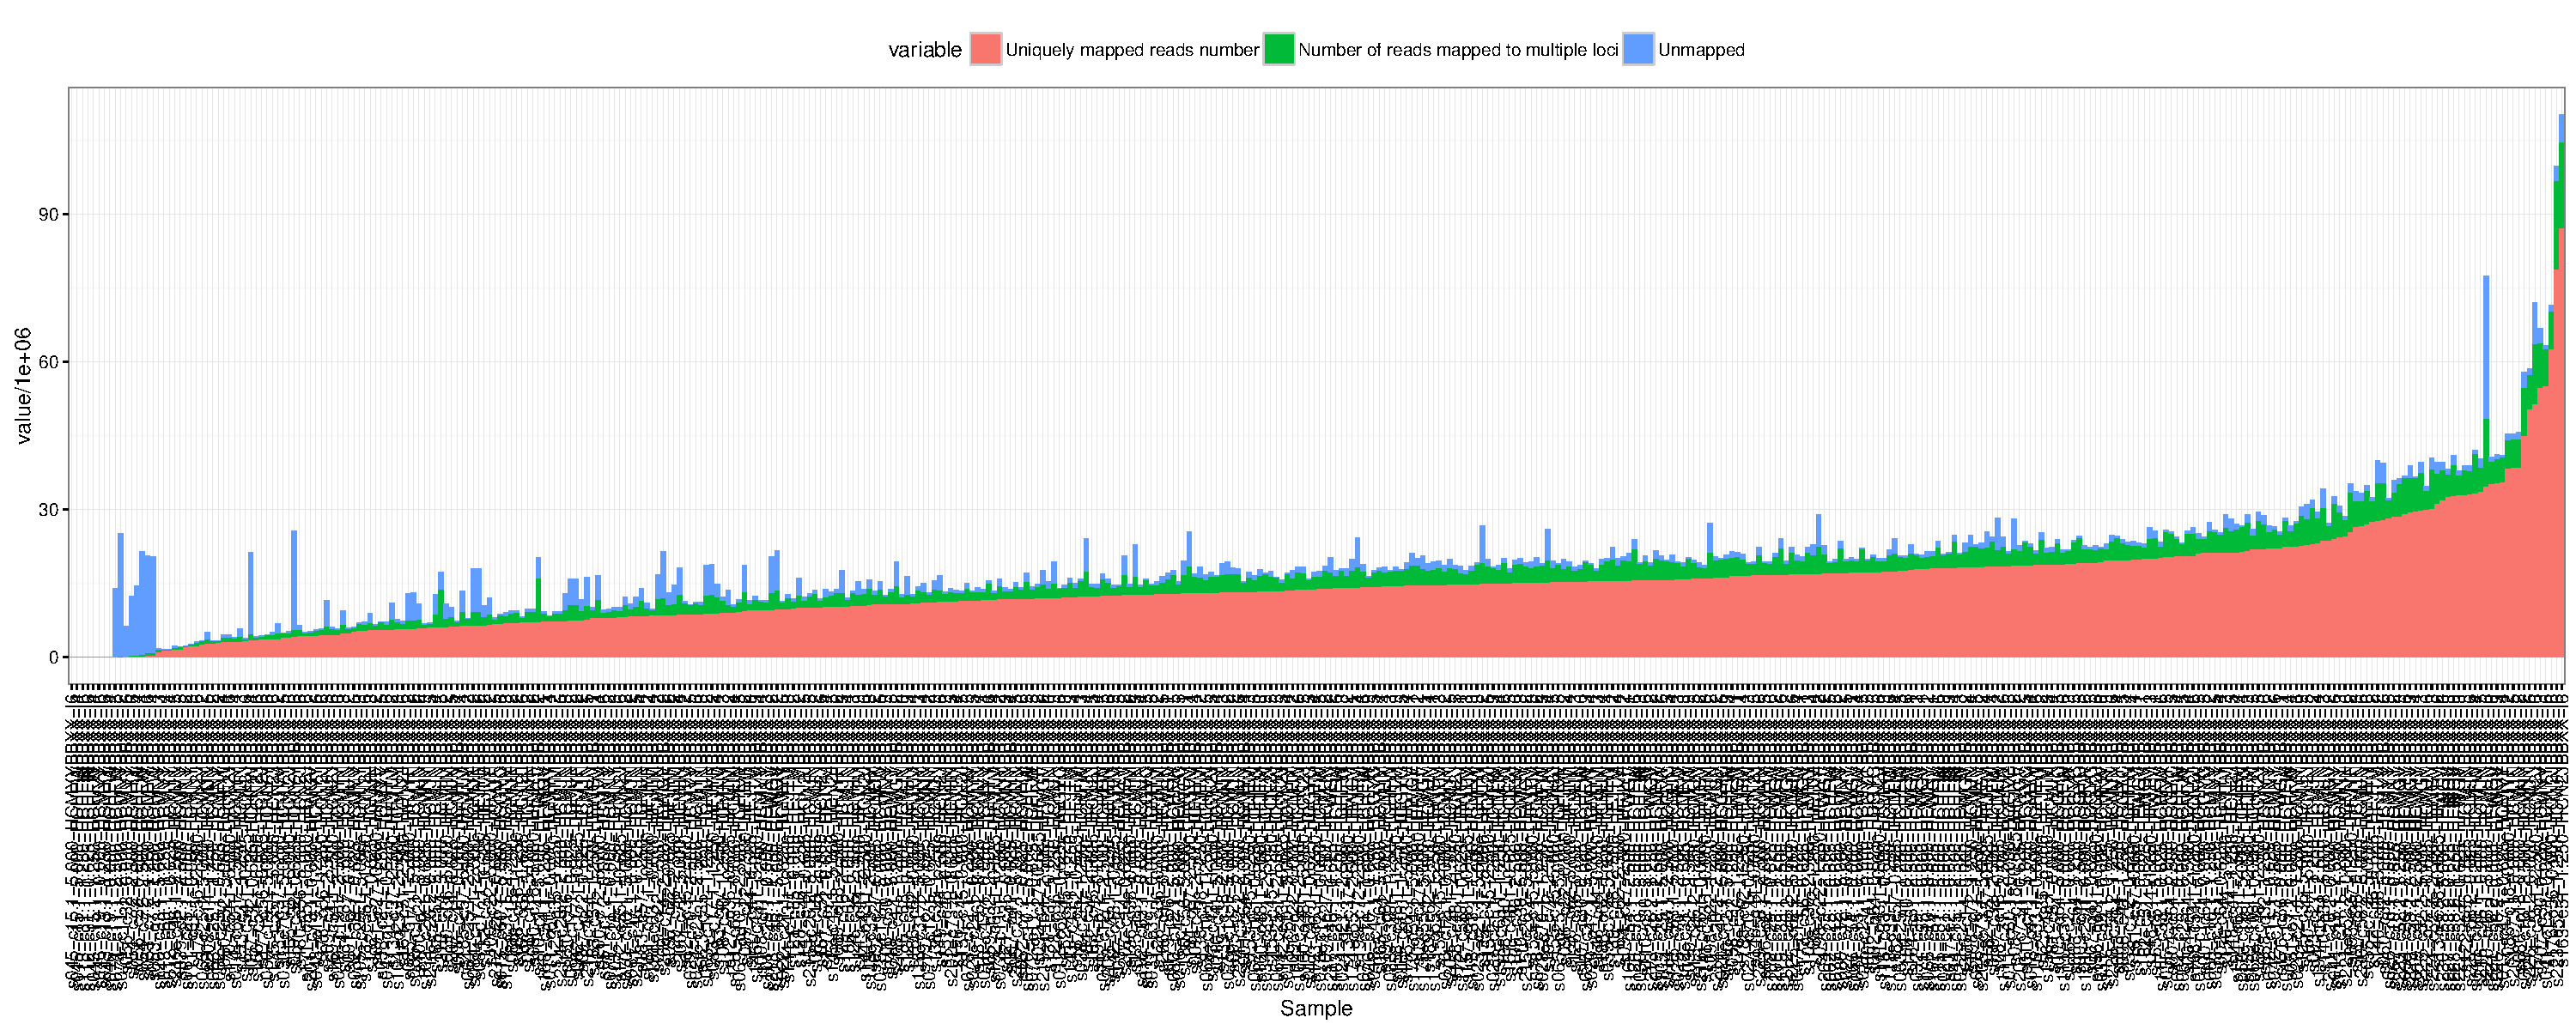
\includegraphics[width=1\textwidth,clip,trim=0 0 0 0]{../figures/mapped.pdf}
\end{frame}

\begin{frame}{Dox conc drives expression variability}
\centering
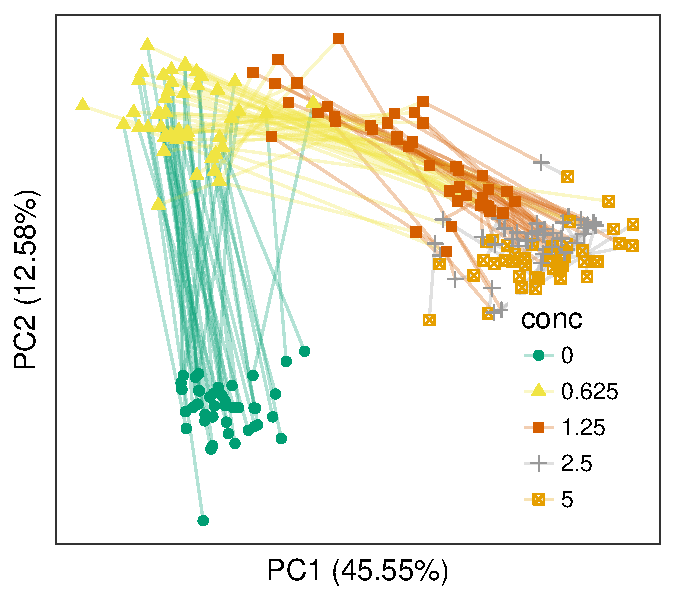
\includegraphics[width=.6\textwidth,clip,trim=0 0 0 0]{../figures/pca.pdf}
\begin{itemize}
\item Expression is \emph{not} linear in dox conc
\item For some individuals $1.25 \sim 0.625$, for others $1.25 \sim 2.5$
\item One clear outlier individual
\end{itemize}
\end{frame}

\begin{frame}{Differential expression}
\begin{itemize}
\item Joint model across concentrations
\end{itemize}
\centering
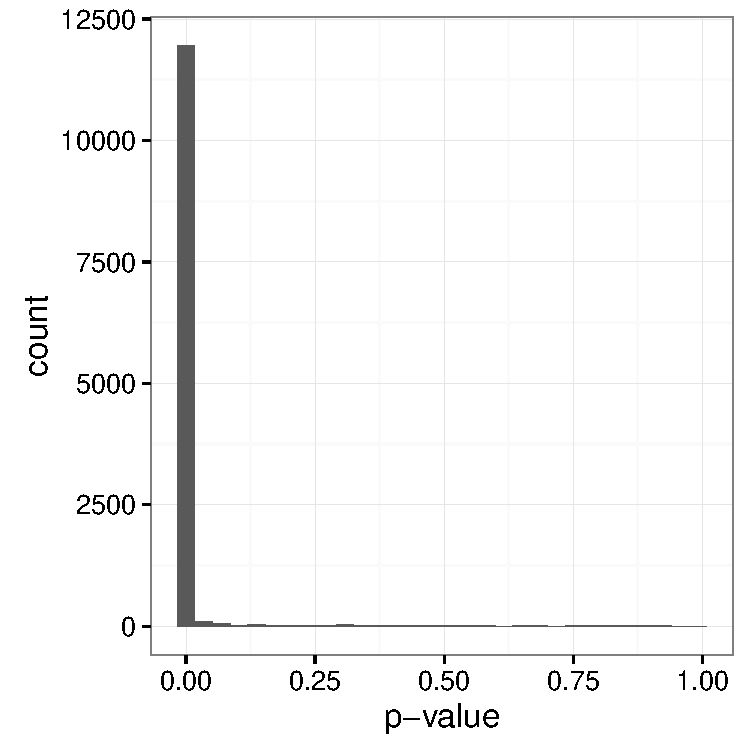
\includegraphics[width=.6\textwidth,clip,trim=0 0 0 0]{../figures/de_boring.pdf}
\begin{itemize}
\item Great... 
\end{itemize}
\end{frame}

\begin{frame}{Response patterns}
\begin{itemize}
\item Cluster genes into response patterns
\end{itemize}
\begin{columns}
\begin{column}{.5\textwidth}
\centering
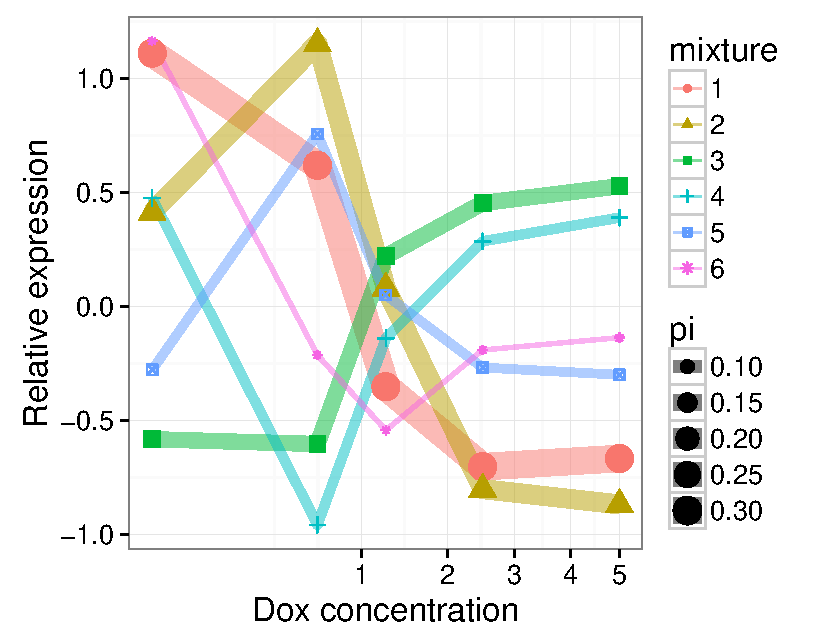
\includegraphics[width=\textwidth,clip,trim=0 0 0 0]{../figures/mixture_centroids.pdf}
\end{column}
\begin{column}{0.5\textwidth}  
\begin{enumerate}
\item Down regulated
\item Initial increase, then decrease
\item Up regulated
\item Transient down regulation
\item Transient up regulation
\item Down regulation and then some recovery. 
\end{enumerate}
\end{column}
\end{columns}
\end{frame}

\begin{frame}{Response pattern model}
\begin{itemize}
\item A $K$-component mixture model with
\begin{align*}
\pi &\sim \text{Dir}(1/K,\cdots,1/K) \\
z_g | \pi &\sim \text{Discrete}(\pi) \\
y_{ngc} | z_g, \theta &\sim N( \theta_{gcz_g}, \sigma^2 )
\end{align*}
\item Marginalize (sum) over $z_g$ and optimize wrt $\pi, \theta, \sigma$ using RStan. 
\end{itemize}
\centering
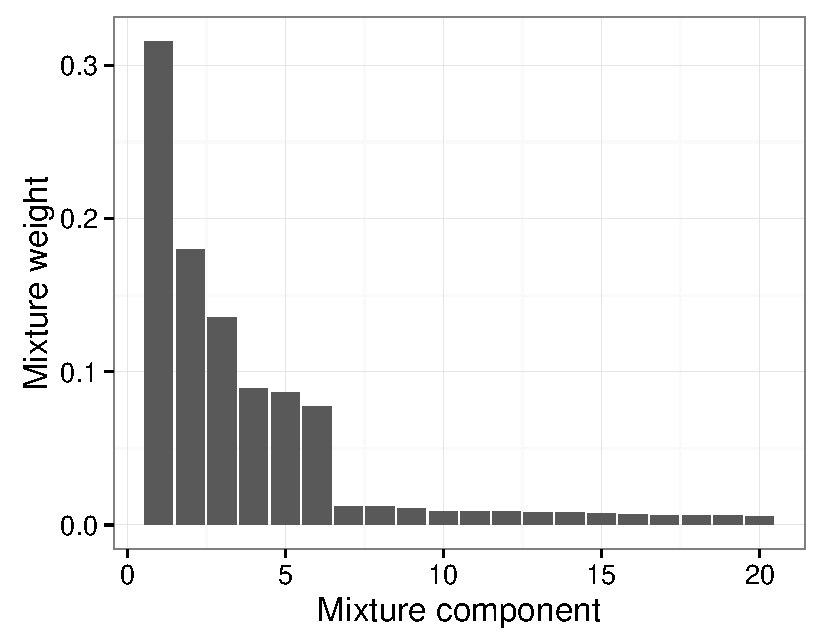
\includegraphics[width=.4\textwidth,clip,trim=0 0 0 0]{../figures/mixture_pi.pdf}
\end{frame}

\begin{frame}{Initial eQTL analysis}
\begin{itemize}
\item Initially using MatrixEQTL - fast and can handle kinship matrix (from IBD)
\item Remove $K$ expression PCs.
\item Include gender as covariate. 
\item Quantile normalize log counts per million. 
\item SNPs within 1Mb, MAF $>5\%$. 
\end{itemize}
\centering
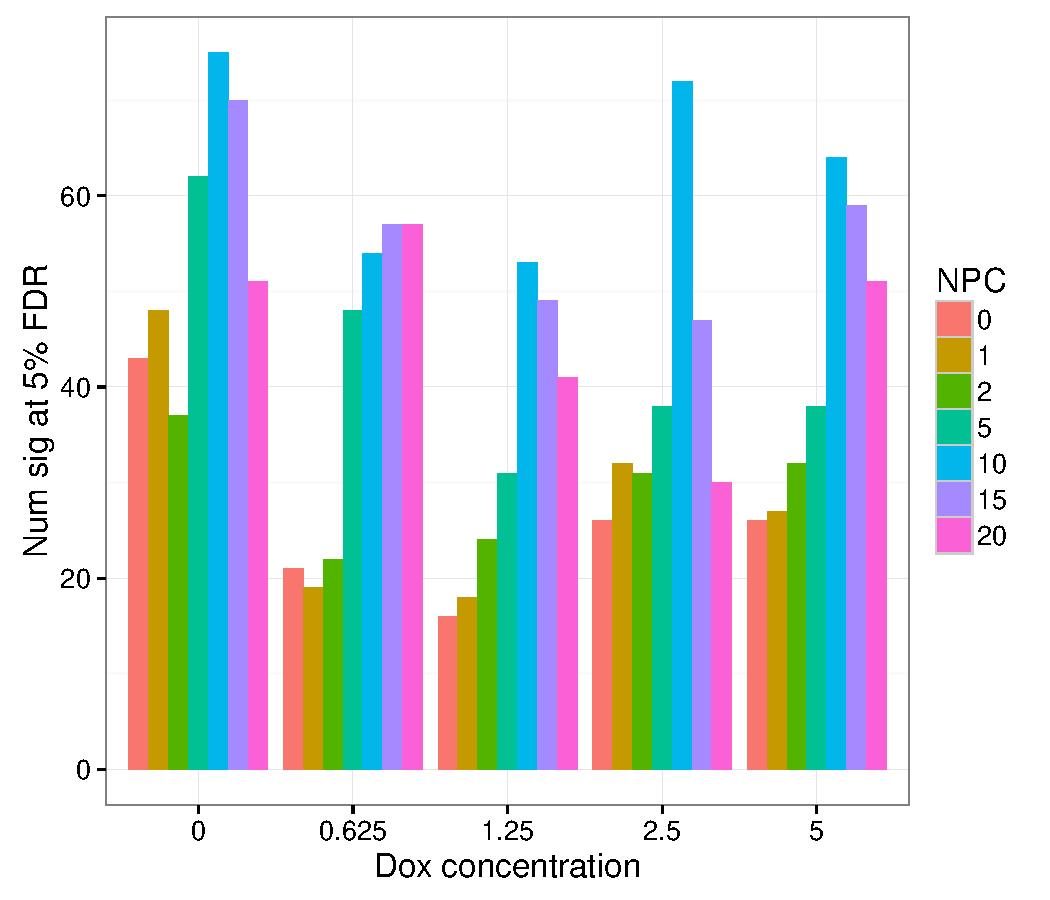
\includegraphics[width=.6\textwidth,clip,trim=0 0 0 0]{../figures/matrixEQTL_nsig.pdf}
\end{frame}

\begin{frame}{Is 75 eQTLs low?}
\begin{itemize}
\item Ignoring the kinship matrix I get 85 (10PCs, no dox)
\item EigenMT \citep{davis2016efficient}: 80
\item Removing 5 genotype PCs: down to 35! 
\item Courtney: ``\emph{Surprisingly, we mapped only 151 eQTLs in this 73 individual LCL panel, less than one-sixth the number of eQTLs we mapped in our panel of iPSC lines}''
\item If only there were some way to improve power...
\end{itemize}
\end{frame}

\begin{frame}{Interaction eQTLs}
\begin{itemize}
\item Started out trying do this with a LMM and REML in R... and got annoyed. 
\item Kinship matrix $\Sigma \rightarrow$ correlated residuals
\item Repeated measurements $\rightarrow$ individual \emph{and} conc level random effect terms
\end{itemize}
\end{frame}


\begin{frame}{Interaction eQTLs}
\begin{align*}
y_{nc} &= \beta g_n + \gamma_c g_n + u_n + v_c + \xi_n + \epsilon_{nc} \\
\beta &\sim N(0, \sigma^2_\beta ) \qquad \textit{ genetic effect }  \\
\gamma_c &\sim N(0, \sigma^2_\gamma ) \qquad \textit{ interaction effects }  \\
u_n &\sim N(0, \sigma^2_u) \qquad \textit{ individual random effects } \\
v_c &\sim N(0, \sigma^2_v)  \qquad \textit{ conc random effect } \\
\xi &\sim MVN(0, \sigma^2_\xi \Sigma ) \qquad \textit{ kinship random effect }  \\
\epsilon &\sim MVN(0, \text{diag}(\sigma^2_\epsilon)) \qquad \textit{ noise } 
\end{align*}
\begin{itemize}
\item Integrate over $\beta, \gamma, u, v, \xi, \epsilon$, optimize the variances $V=\{ \sigma^2_\beta, \sigma^2_\gamma,  \sigma^2_u, \sigma^2_v,  \sigma^2_\xi, \sigma^2_\epsilon \}$
\item Null hypothesis: $\sigma^2_\gamma = 0$. Alternative: $\sigma^2_\gamma > 0$.
\item Look for
$
L=\log\frac{ \max_V P( y | V ) }{ \max_{V \backslash \sigma^2_\gamma} P(y | V, \sigma^2_\gamma=0 ) }
L > 10$, roughly $ \sim p < 0.001$. 
\end{itemize}
\end{frame}

\begin{frame}{Sensitizing}
\centering
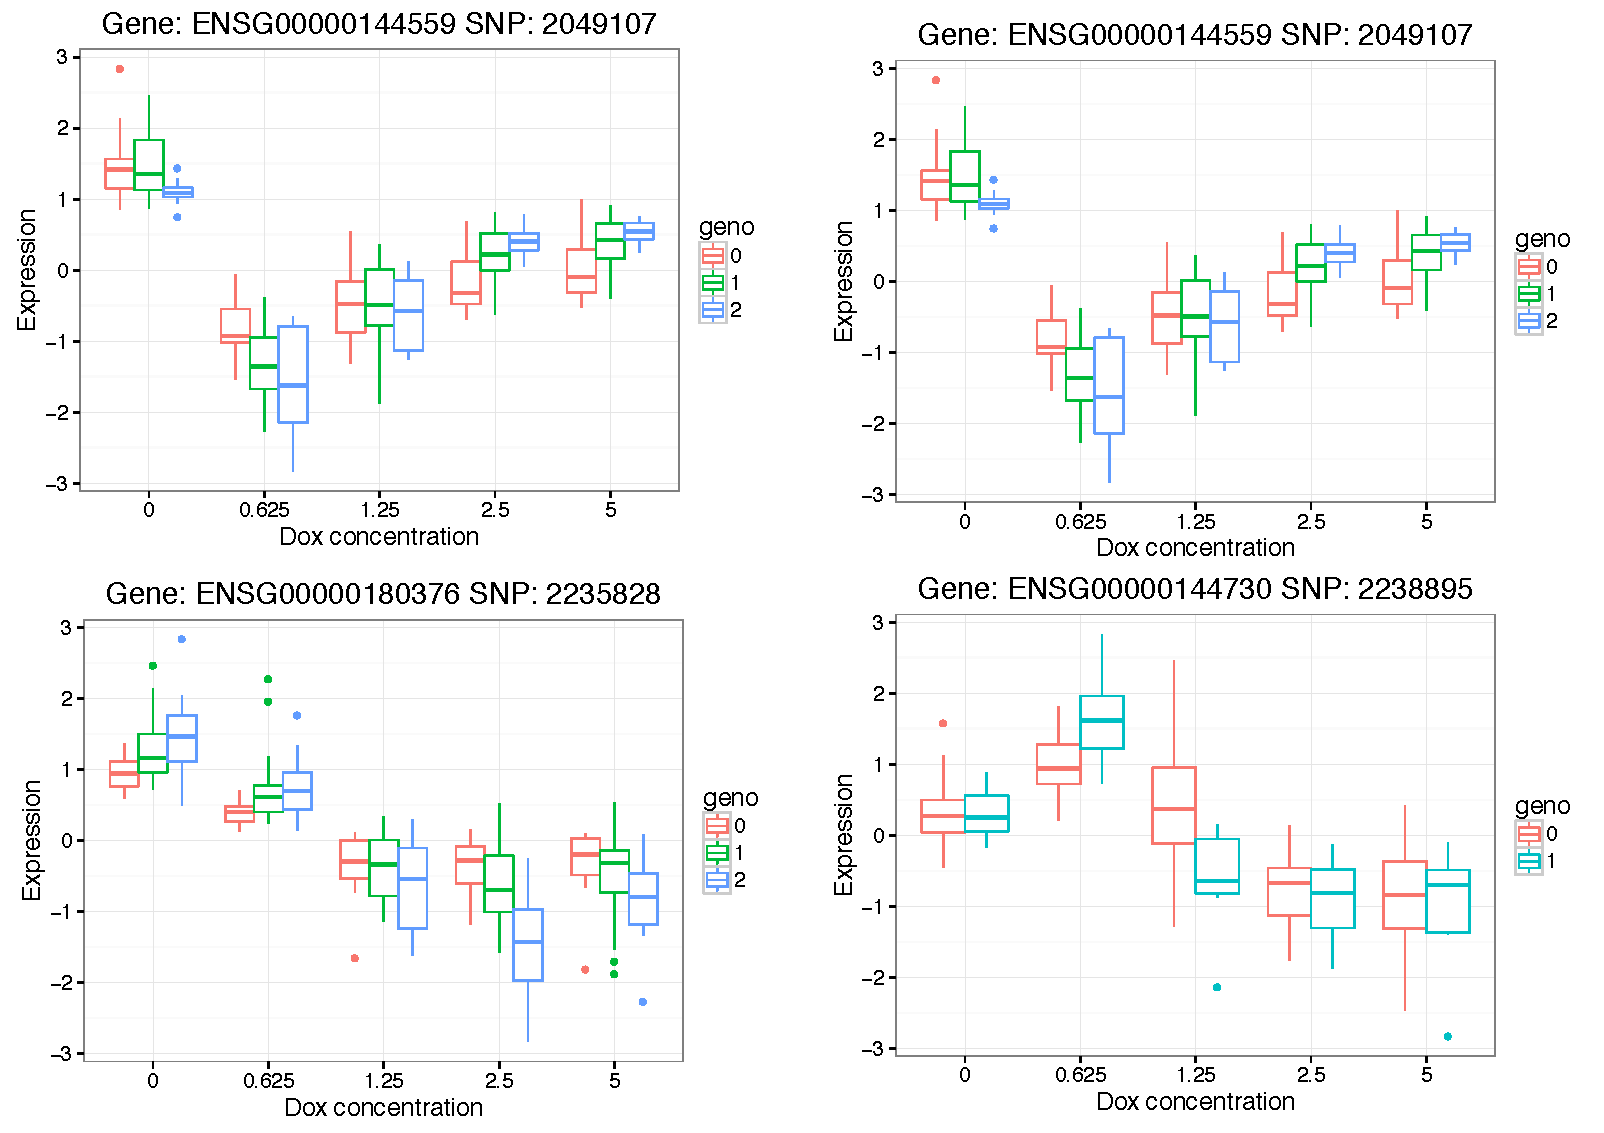
\includegraphics[width=\textwidth,clip,trim=0 0 0 0]{../figures/iqtl_types/sensitizing.pdf}
\end{frame}

\begin{frame}{De-sensitizing}
\centering
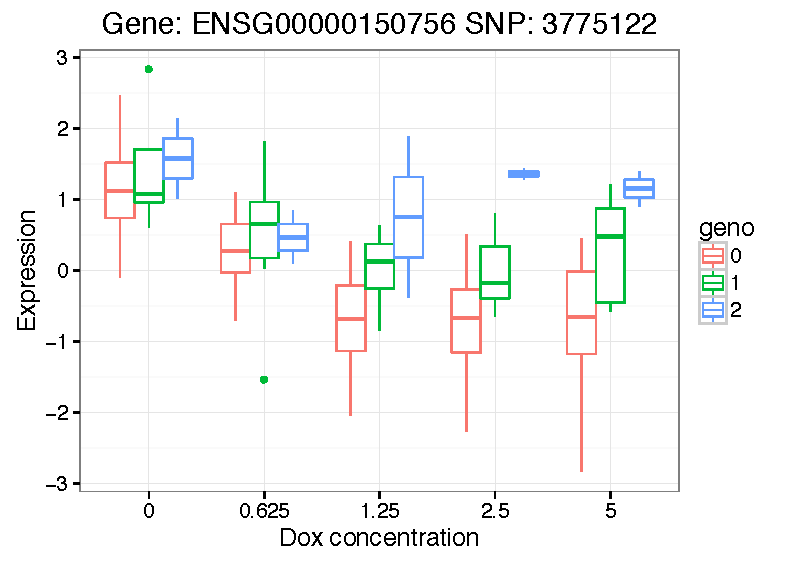
\includegraphics[width=\textwidth,clip,trim=0 0 0 0]{../figures/iqtl_types/desensitizing.pdf}
\end{frame}

\begin{frame}{Extreme sensitizing?}
\centering
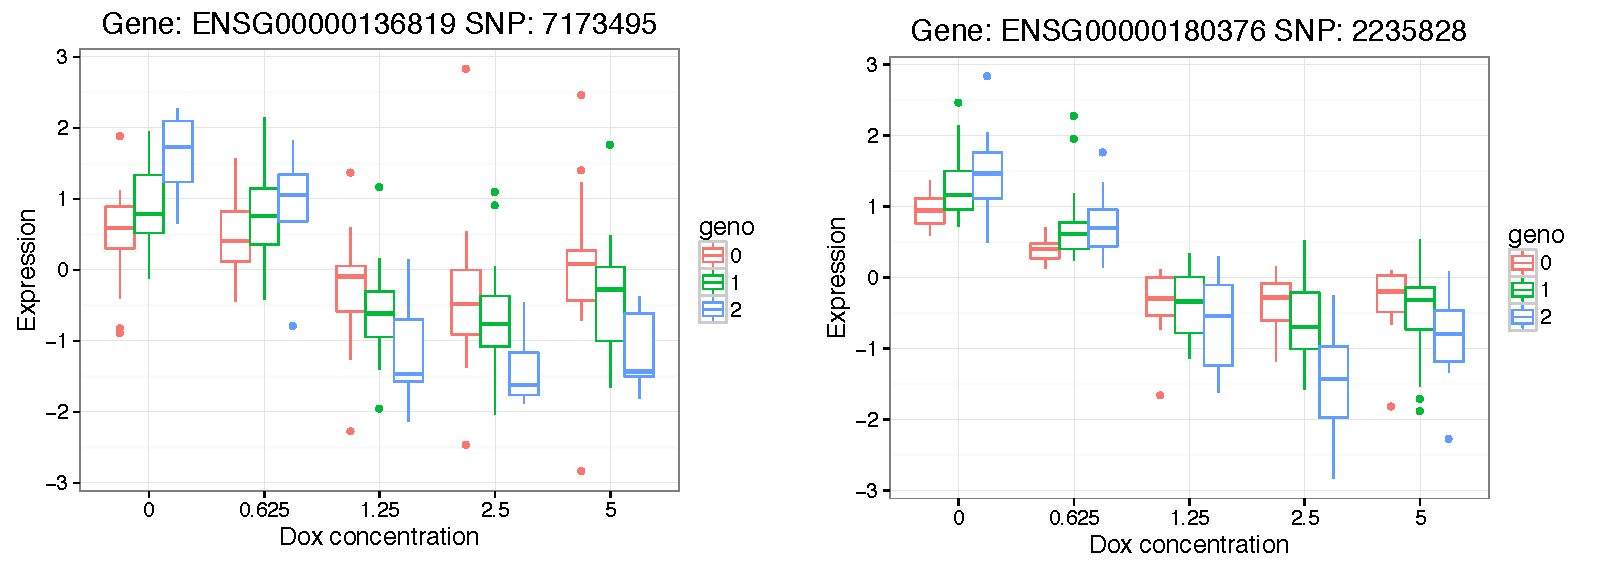
\includegraphics[width=\textwidth,clip,trim=0 0 0 0]{../figures/iqtl_types/extreme.pdf}
\end{frame}

\begin{frame}{Opposite effect}
\centering
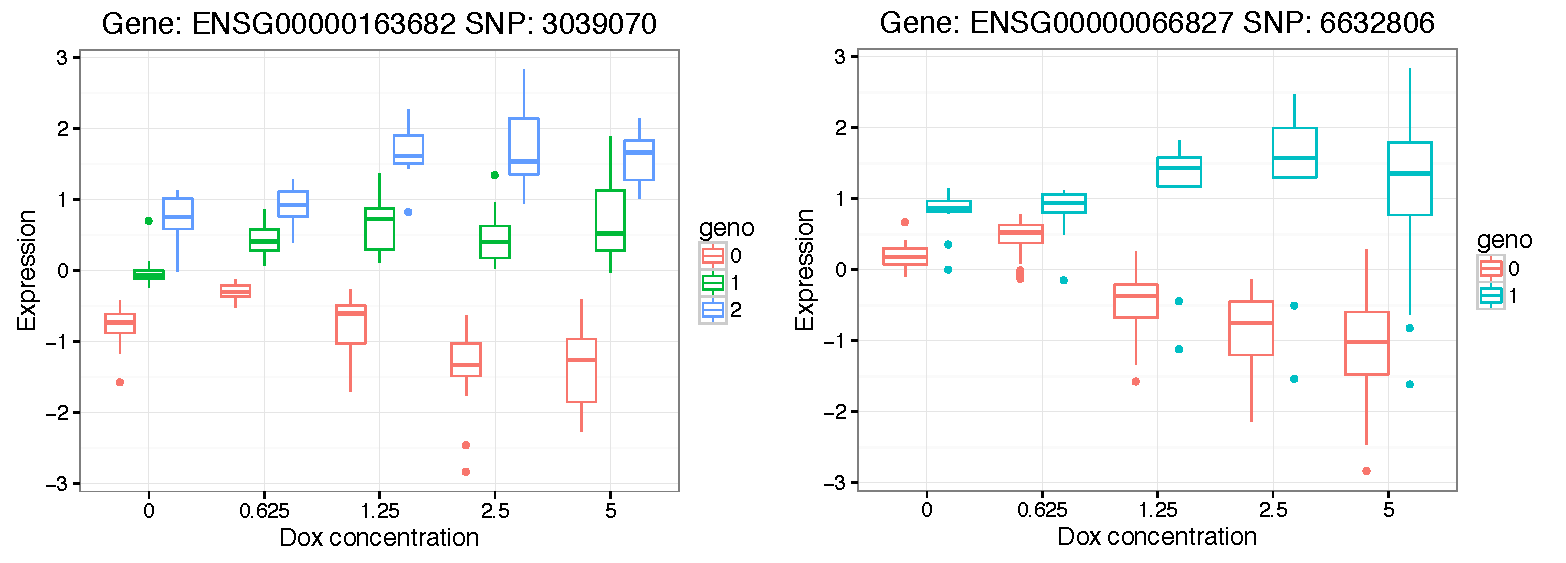
\includegraphics[width=\textwidth,clip,trim=0 0 0 0]{../figures/iqtl_types/opposite_effect.pdf}
\end{frame}

\begin{frame}{Buffering?}
\centering
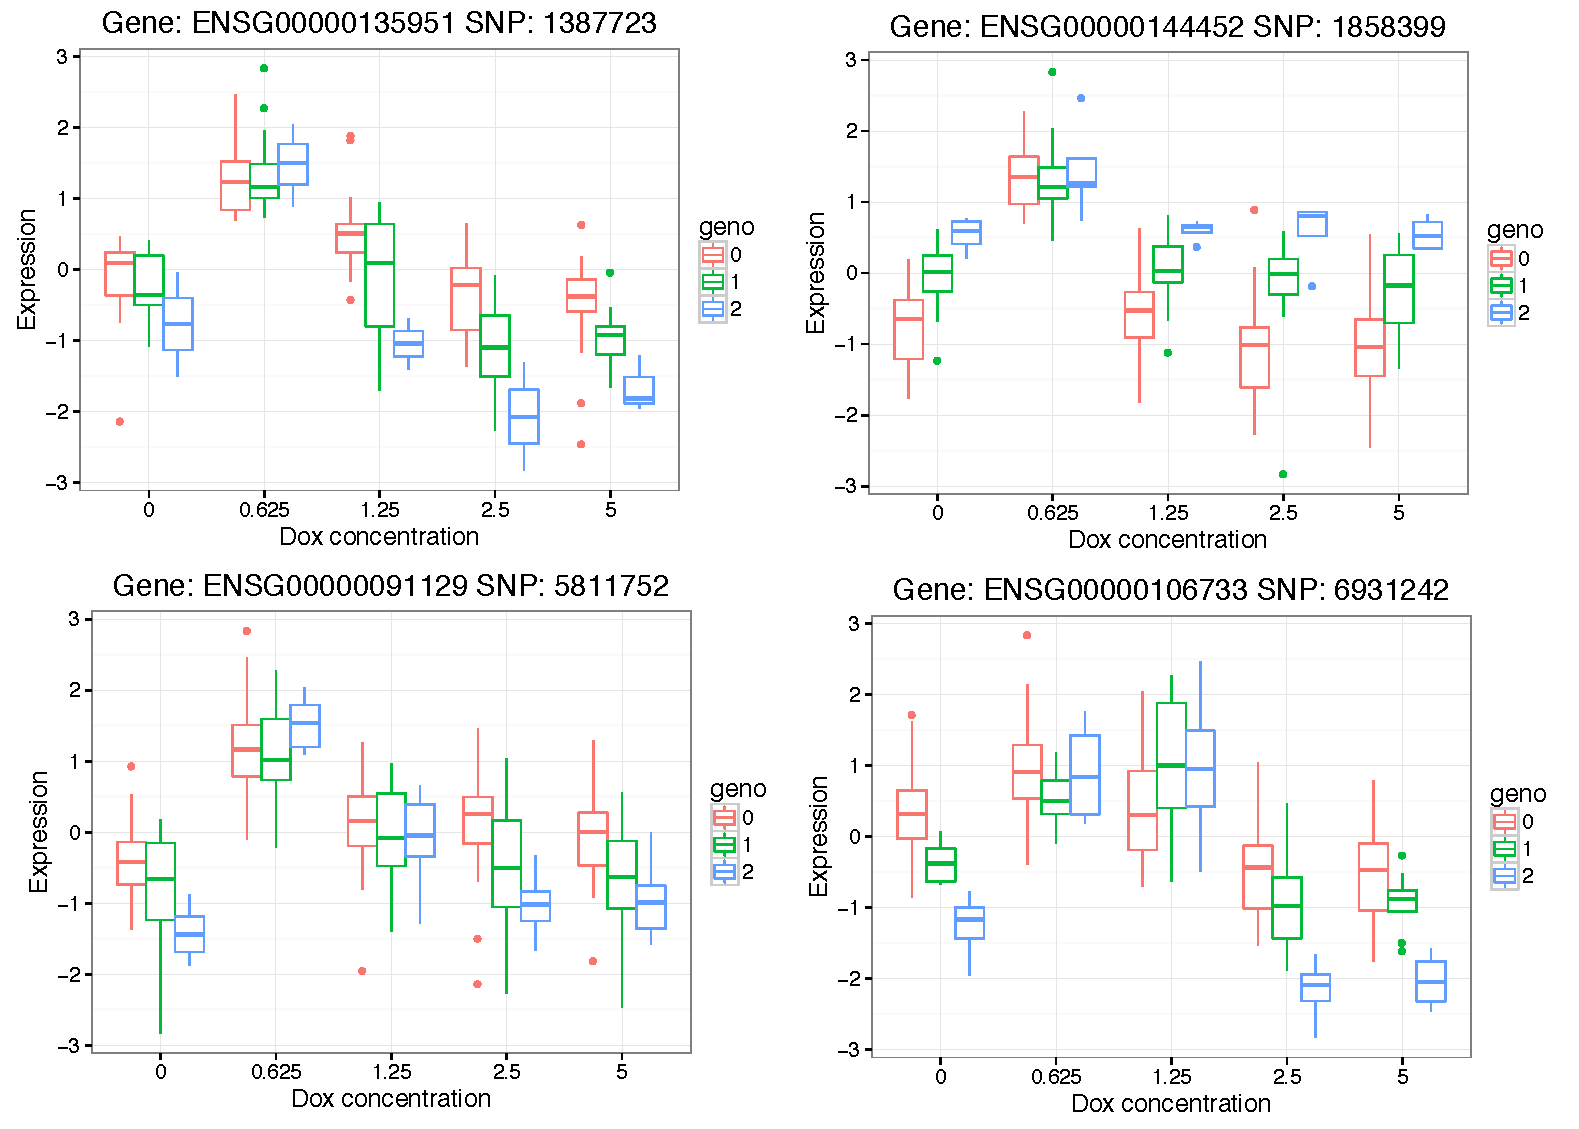
\includegraphics[width=\textwidth,clip,trim=0 0 0 0]{../figures/iqtl_types/buffering.pdf}
\end{frame}

\begin{frame}{Troponin}
\begin{itemize}
\item Used as a blood borne marker of cardiac damage
\end{itemize}
\centering
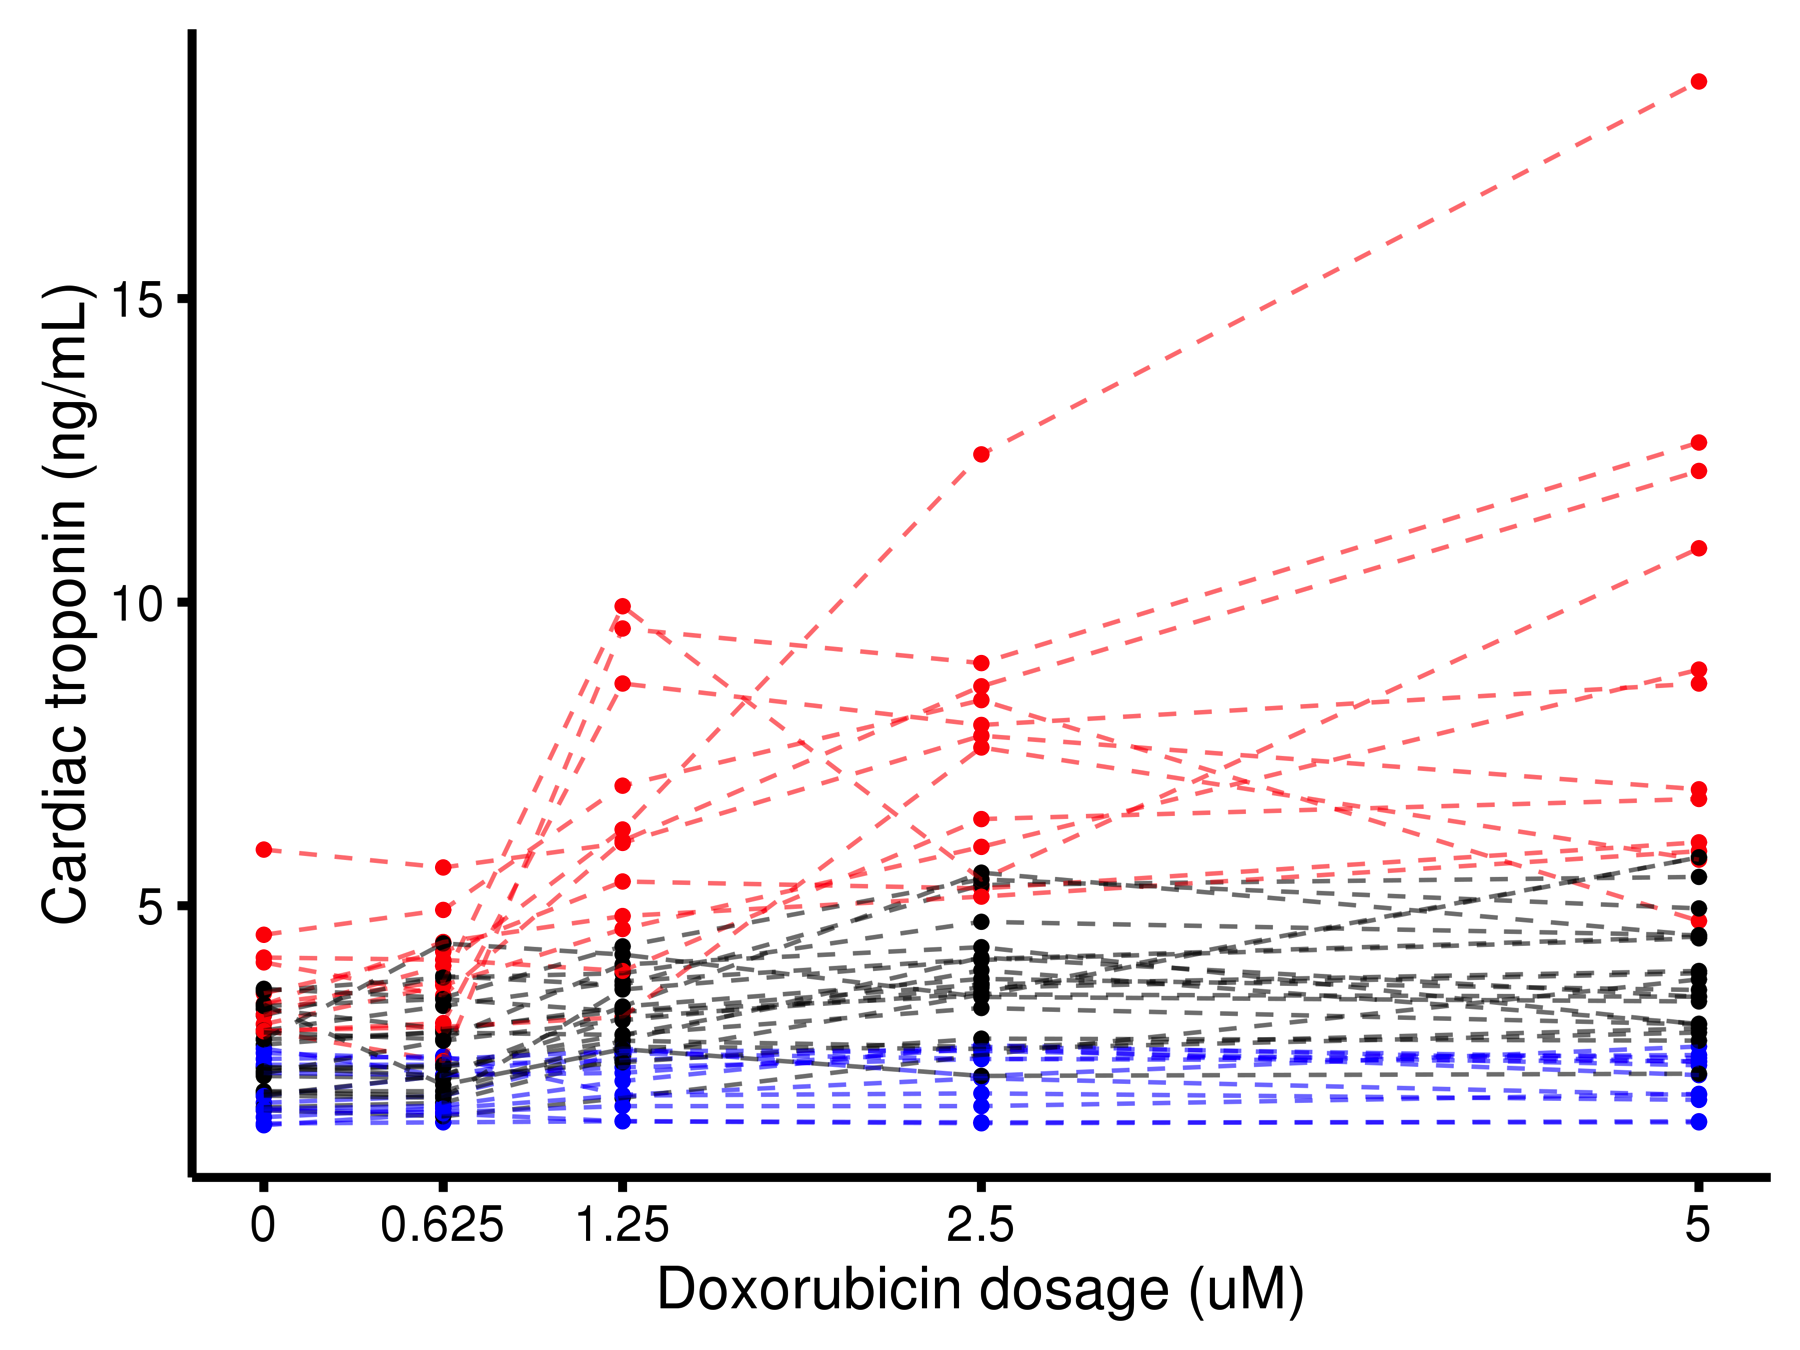
\includegraphics[width=\textwidth,clip,trim=0 0 0 0]{../figures/troponin.png}
\end{frame}

\begin{frame}{Ideas/todo}
\begin{itemize}
\item Using allelic signal to improve power (challenging for iQTLs)
\item Link to clinical variables and troponin response
\item Look for TF motifs explaining iQTLs
\item Splicing (obviously)
\item Unfortunately I can't find a GWAS for dox cardiotoxicity sensivitiy...
\end{itemize}
\end{frame}

\begin{frame}[allowframebreaks]{Bibliography}
\small
\def\newblock{}
\bibliography{dox}
\bibliographystyle{apa}
\end{frame}


\end{document}
